\documentclass[11pt]{article}
% =====================================================================
%  VP-pro family --- the four program-feature categories, explained.
%  Companion to i2s_pro_categories.tex / i2s_anti_categories.tex.
%  Every cited branch + value is REAL (bench/dataset.jsonl + per-branch
%  cards). lcms/libxml2/libpng gates verified against local source dumps;
%  harfbuzz/sqlite3 gates from their cards (corpora on the other server).
%  Compile: pdflatex vp_pro_categories.tex   (needs tikz + pgfplots + listings)
% =====================================================================
\usepackage[margin=1in]{geometry}
\usepackage{amsmath,amssymb}
\usepackage{xcolor}
\usepackage{listings}
\usepackage{booktabs}
\usepackage{tikz}
\usepackage{pgfplots}
\pgfplotsset{compat=1.16}
\usetikzlibrary{arrows.meta,positioning,shapes.geometric}

\definecolor{winc}{RGB}{30,120,60}   % winner (value_profile resolves) green
\definecolor{losc}{RGB}{190,60,60}   % loser  (no VP gradient)         red
\definecolor{codebg}{RGB}{246,246,248}
\definecolor{kw}{RGB}{40,60,150}
\definecolor{cmt}{RGB}{120,120,120}
\definecolor{str}{RGB}{160,60,20}

\lstdefinestyle{c}{
  language=C, basicstyle=\ttfamily\small, backgroundcolor=\color{codebg},
  keywordstyle=\color{kw}\bfseries, commentstyle=\color{cmt}\itshape,
  stringstyle=\color{str}, numbers=none, frame=single, framerule=0pt,
  framesep=6pt, breaklines=true, showstringspaces=false, xleftmargin=4pt,
}

% A small "metric & rule" box used under every category.
\newcommand{\metricbox}[4]{%
  % #1 tool  #2 metric (plain meaning)  #3 verify rule  #4 real example
  \par\smallskip\noindent\fbox{\parbox{\dimexpr\linewidth-2\fboxsep-2\fboxrule}{%
  \footnotesize
  \textbf{Tool:}~\texttt{#1}\\[2pt]
  \textbf{Metric:}~#2\\[2pt]
  \textbf{Verify rule (the arbiter fires this, no LLM):}~\texttt{#3}\\[2pt]
  \textbf{Real example:}~#4}}\par\smallskip}

\title{\textbf{The VP-pro family: four reasons the value-profile gradient gets through}}
\author{}
\date{}

\begin{document}
\maketitle
\vspace{-3em}

\paragraph{Backdrop.} \emph{VP-pro} collects the roadblocks where a fuzzer that
\emph{scores how byte-close each comparison came} (value\_profile's
Hamming-similarity / \texttt{CMP\_MAP} feedback) gets through, while a fuzzer
without that gradient stays stuck. Where I2S needs the right value to be lying
around so it can \emph{paste} it, VP needs no such luck: each comparison emits a
\emph{partial-match} reward that turns a flat ``wrong/right'' cliff into a hill
the fuzzer can climb one byte at a time. Picture a combination lock that clicks
louder as each wheel nears its number --- VP hears the clicks and turns toward
them; plain havoc (and even exact-paste I2S, when the value is \emph{not} already
in the corpus) has no slope to follow. All the categories below share that
gradient --- they differ in \emph{what} the climb buys. Counts are validated
roadblocks ($n$); a branch joins VP-pro by its \emph{deciding pair}
(value\_profile resolves, its non-VP partner blocks), not by the raw 4-char shape.

% =====================================================================
\section*{1.\ \ Operand byte-gradient climb \hfill {\normalsize\texttt{vp\_gradient\_value\_distance\_closure} ($n=33$)}}
The dominant case. The gate is an exact multi-byte compare (a FourCC tag, a
keyword, a magic constant). The non-VP arm's best seed gets \emph{some} of the
bytes right and stalls there --- it has no signal telling it the remaining bytes
are wrong-but-close. The value-profile gradient scores that near-match, so VP
keeps the partial hit and climbs the last bytes home. \emph{It is not getting to
the door; it is hearing the lock click toward open.}

\begin{lstlisting}[style=c]
// lcms  cmspcs.c : cmsChannelsOfColorSpace()
// dispatch on the 4-byte ICC colour-space signature
switch (ColorSpace) {
case cmsSigMCH2Data:                  // <-- blocker (lcms/2288): sig == 'MCH2'
case cmsSig2colorData:  return 2;     //     needs all four exact bytes
}
\end{lstlisting}

\noindent\textbf{How we know it is really the gradient.} We measure how
\emph{close} each side's nearest seed gets to the target operand (a normalised
Hamming distance, $0$ = exact hit). The non-VP arm stalls at a positive residual;
the value\_profile arm closes it.

\metricbox{value\_distance\_reached}
{\texttt{naive\_min\_distance} = the non-VP arm's residual to the operand ($>0$ = never lands it); \texttt{distance\_gap} = how much further from the operand the loser stalls; \texttt{distance\_closure\_ratio} = fraction of that gap VP closes; \texttt{winner\_closer} (bool)}
{winner\_closer == true AND distance\_gap >= 0.15}
{lcms/2288 (\texttt{cmsChannelsOfColorSpace}, operand \texttt{'MCH2'}) --- the non-VP arm stalls at distance $0.75$ (one of four bytes right); value\_profile reaches $0.0$, so \texttt{distance\_gap}$=0.75$ and \texttt{distance\_closure\_ratio}$=1.0$ (closes the whole gap).}

\begin{center}
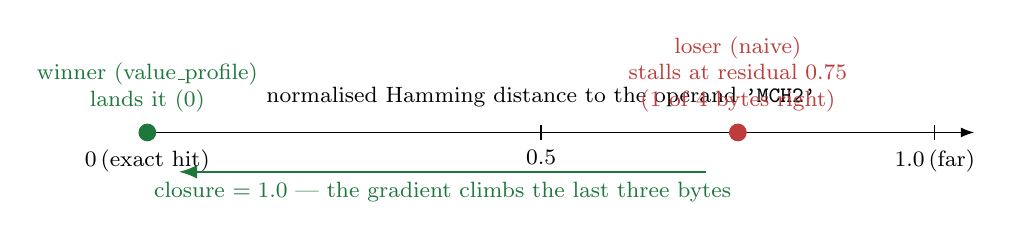
\begin{tikzpicture}[font=\footnotesize,>=Latex]
\draw[->] (0,0) -- (10.5,0);
\foreach \x/\l in {0/0\,(exact hit), 5/0.5, 10/1.0\,(far)} \draw (\x,0.1)--(\x,-0.1) node[below]{\l};
\node[above] at (5,0.2) {normalised Hamming distance to the operand \texttt{'MCH2'}};
% loser marker at 0.75 -> x = 7.5
\filldraw[losc] (7.5,0) circle (3pt) node[above=4pt,losc,align=center]{loser (naive)\\stalls at residual $0.75$\\(1 of 4 bytes right)};
% winner marker at 0
\filldraw[winc] (0,0) circle (3pt) node[above=4pt,winc,align=center]{winner (value\_profile)\\lands it ($0$)};
\draw[->,winc,thick] (7.1,-0.5) -- (0.4,-0.5) node[midway,below]{closure $=1.0$ --- the gradient climbs the last three bytes};
\end{tikzpicture}\\[2pt]
{\footnotesize Without a gradient the loser cannot tell ``one byte right'' from ``none right''; VP's per-byte score gives it the slope to finish.}
\end{center}

\paragraph{Sub-case: the operand sits at a FIXED offset (enrichment route).}
Five of these branches gate on a magic value at a \emph{fixed} file offset --- an
ICC device-class signature, a FourCC, a size tag --- so instead of a
sliding-window distance we measure the same climb directly as byte
\emph{enrichment} at that offset: value\_profile ratchets the corpus until the
exact operand bytes pile up there (the end-state I2S reaches by pasting, arrived
at by climbing). The mechanism is identical to the distance route above; only the
measurement is anchored to the offset --- exactly the dual measurement route
\texttt{i2s\_string\_literal\_substitution} uses (enrichment when the literal has a
fixed offset, distance when it floats). These \texttt{LWWL}/\texttt{L\_WL} branches
typically resolve under I2S too --- the boundary where VP-pro touches I2S-pro ---
so the enrichment is a \texttt{cmplog}-vs-\texttt{naive} ratio and the VP
attribution comes from the deciding pair.

\metricbox{operand\_enrichment}
{\texttt{signed\_target\_enrich} $=\log_2\!\frac{\text{corpus freq}+\epsilon}{\text{baseline freq}+\epsilon}$ at the gate offset ($>0$ = the exact bytes piled up there); \texttt{decoy\_enrich} (the competing value)}
{signed\_target\_enrich >= 1.0 AND decoy\_enrich < signed\_target\_enrich}
{lcms/2143 (\texttt{validDeviceClass}, ICC device-class signature at offset \texttt{0x0C}) --- \texttt{signed\_target\_enrich}$=+17.85$, \texttt{decoy\_enrich}$=-0.90$: the exact class bytes pile up at the offset while the wrong classes drain. Same ICC-header gate family as the \texttt{'MCH2'} example above, neighbouring offset --- which is why splitting them by measurement tool was an artefact.}

% =====================================================================
\section*{2.\ \ The gradient builds more structure: assembly depth \hfill {\normalsize\texttt{vp\_gradient\_assembly\_depth} ($n=20$)}}
Where category~1's gradient closes the distance to one \emph{value}, this
category's gradient produces more \emph{structure} on the way to the gate. It has
\textbf{two measurement routes} --- the same two the joint family's
\texttt{joint\_assembly\_depth} bundles, here for a single technique: VP either
drives the parser \emph{deeper} per seed (route~A, \texttt{depth\_reach}) or admits
a \emph{larger / token-denser} valid corpus (route~B,
\texttt{struct\_size\_and\_token\_count}). Both are ``more structure assembled'';
which route fires is a property of the gate, not a different mechanism. (We earlier
split these as two categories --- \emph{drives\_assembly\_depth} ($15$) and
\emph{admits\_structurally\_richer\_corpus} ($5$) --- but \emph{size} alone cannot
separate ``drives \emph{this} gate deeper'' from ``admits a bigger corpus in
general'' (and size is already route~B's metric), so they are one mechanism with
two routes, merged 2026-06-26.)

\paragraph{Route A --- drives the parser deeper (depth).} The climb is \emph{along
a chain}: each loop iteration or nested field has its own comparison, and VP's
per-comparison reward keeps rewarding seeds that get one step further in, marching
the parser \emph{deeper} until it reaches the gate. The tell is not ``the right
bytes are present'' --- it is ``the VP seeds execute the blocker line far more /
drive it much further in.''

\begin{lstlisting}[style=c]
// libxml2  parser.c : xmlParseCharRef()   (numeric char-ref  &#NN;)
} else if ((RAW == '&') && (NXT(1) == '#')) {
    SKIP(2);
    while (RAW != ';') {              // <-- blocker (libxml2/6466): digit-assembly loop
        if ((RAW >= '0') && (RAW <= '9'))   //     each pass consumes one more digit
            val = val * 10 + (RAW - '0');
        NEXT;
    }
}
\end{lstlisting}

\noindent\textbf{How we know.} We run each side's corpus and count, per seed, how
many times the blocker line executes (its parse \emph{depth}) and whether the seed
takes the decisive side. The VP arm should reach the line far more.

\metricbox{depth\_reach}
{\texttt{depth\_lift} = winner / loser per-seed executions of the blocker line; \texttt{side\_lift} = how much more the winner takes the decisive branch; \texttt{winner\_deeper} (bool)}
{depth\_lift >= 1.5 AND winner\_deeper == true}
{libxml2/6466 (\texttt{xmlParseCharRef}, the \texttt{while (RAW != ';')} digit loop, \texttt{parser.c:2352}) --- \texttt{depth\_lift}$=9.07$, \texttt{side\_lift}$=7.8$: the value\_profile corpus drives the char-ref assembly loop ${\approx}9\times$ deeper per seed than its non-VP partner.}

\begin{center}
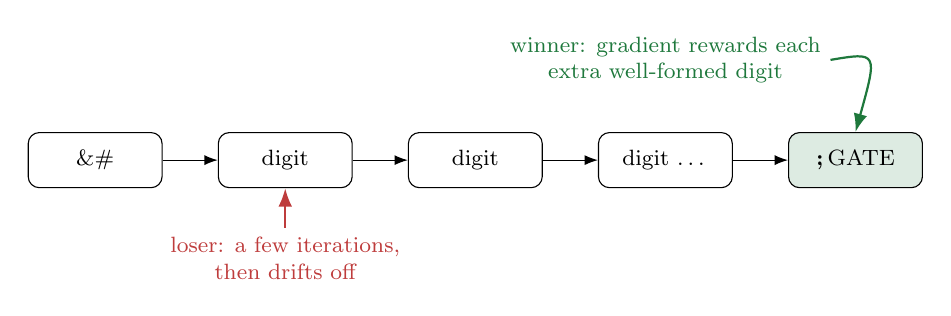
\begin{tikzpicture}[font=\footnotesize,>=Latex,node distance=7mm]
\tikzstyle{f}=[draw,rounded corners,minimum width=17mm,minimum height=7mm]
\node[f] (a) {\&\#};
\node[f,right=of a] (b) {digit};
\node[f,right=of b] (c) {digit};
\node[f,right=of c] (d) {digit \dots};
\node[f,right=of d,fill=winc!15] (e) {\textbf{;}\,GATE};
\draw[->] (a)--(b); \draw[->] (b)--(c); \draw[->] (c)--(d); \draw[->] (d)--(e);
% loser stalls shallow
\node[losc,below=5mm of b,align=center] (l) {loser: a few iterations,\\then drifts off};
\draw[->,losc,thick] (l) -- (b.south);
% winner reaches gate
\node[winc,above=5mm of d,align=center] (w) {winner: gradient rewards each\\extra well-formed digit};
\draw[->,winc,thick] (w.east) .. controls +(0.6,0.1) .. (e.north);
\end{tikzpicture}\\[2pt]
{\footnotesize Each comparison on the chain emits its own partial-match reward, so VP's corpus keeps walking deeper; the loser has no slope past the first steps.}
\end{center}

% =====================================================================
\paragraph{Route B --- admits a larger / token-denser corpus (size).} The other
route to ``more structure'' (the $5$ branches formerly labelled
\emph{admits\_structurally\_richer\_corpus}): extra valid structure (a longer
well-formed body, more keywords/tokens) opens \emph{more} comparison gradients
downstream --- so VP's feedback rewards seeds that carry it, and the whole corpus
drifts toward \emph{bigger} or \emph{more token-dense} valid inputs. The non-VP arm
has no reason to grow its seeds, so it never accumulates the structure the gate
needs. Two measurable sub-signals: more total valid \emph{size}, or higher
\emph{token density}.

\begin{lstlisting}[style=c]
// a downstream gate only longer / token-dense valid inputs reach
parse_header(in);                 // every arm clears this
... build_body(in) ...            // VP's corpus grows larger valid bodies here
if (have_enough_structure(in))    // <-- blocker: only the richer corpus arrives
    enter_deep_state(in);
\end{lstlisting}

\noindent\textbf{How we know.} We compare the winner's and loser's seed sets for
this branch on two structural axes --- mean valid \emph{size} and \emph{token
density} --- and require the VP side to be richer.

\metricbox{struct\_size\_and\_token\_count}
{\texttt{size\_lift} = winner / loser mean valid size; \texttt{tag\_lift} = relative count of structural tags; \texttt{token\_density\_lift} = winner / loser tokens-per-byte}
{(size\_lift >= 1.3 AND tag\_lift >= 1.0) OR (token\_density\_lift >= 2.0 AND vp\_token\_density > naive\_token\_density)}
{harfbuzz/5302 --- \texttt{size\_lift}$=4.69$ (VP seeds average $258$ B vs $55$ B), \texttt{tag\_lift}$=1$: the VP corpus carries a much larger valid font body. Token-density sub-case sqlite3/14588 --- \texttt{token\_density\_lift}$=34.6$ ($0.154$ vs $0.004$ tokens/byte): VP's corpus is far more SQL-token-dense.}

\begin{center}
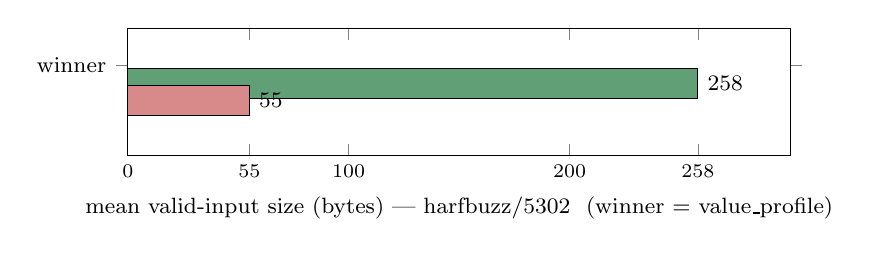
\begin{tikzpicture}
\begin{axis}[
  width=10cm, height=3.2cm, xbar, xmin=0, xmax=300,
  bar width=11pt, enlarge y limits=0.7,
  symbolic y coords={loser, winner},
  ytick=data, yticklabel style={font=\footnotesize}, xtick={0,55,100,200,258},
  xticklabel style={font=\scriptsize},
  nodes near coords, every node near coord/.append style={font=\footnotesize},
  xlabel={\footnotesize mean valid-input size (bytes) --- harfbuzz/5302 \ (winner = value\_profile)},
]
\addplot[fill=winc!70] coordinates {(258,winner)};
\addplot[fill=losc!60] coordinates {(55,loser)};
\end{axis}
\end{tikzpicture}\\[-1pt]
{\footnotesize VP rewards the extra structure that opens further gradients, so its corpus grows the valid body ($\texttt{size\_lift}=4.69$); the loser stays small.}
\end{center}

% =====================================================================
\section*{3.\ \ Incremental conjunction climb \hfill {\normalsize\texttt{vp\_incremental\_conjunction\_climb} (a \emph{recovered} category)}}
The category the automated pipeline \emph{missed}. The gate is not one multi-byte
compare but a \emph{conjunction} of $\ge 2$ narrow equality checks against
constants that together form a contiguous magic / signature / byte-order mark
(BOM): \texttt{if (b[0]==C$_0$ \&\& b[1]==C$_1$ \&\& $\dots$)}. value\_profile
climbs it \emph{one clause at a time} --- each \texttt{\&\&} term emits its own
\texttt{CMP\_MAP} partial-match reward \emph{and} its own short-circuit coverage
edge --- so its corpus reaches a deeper prefix of the sequence than the loser,
which substitutes/guesses one operand at a time and stalls partway. This is
exactly the paper's motivating example (Fig.~2a):

\begin{lstlisting}[style=c]
// libxml2  encoding.c : xmlDetectCharEncoding()  -- recognise a UCS-4 BOM
if ((in[0] == 0x00) && (in[1] == 0x00) &&
    (in[2] == 0x00) && (in[3] == 0x3C))      // <-- blocker (libxml2/6337)
    return(XML_CHAR_ENCODING_UCS4BE);        //     value_profile resolves 9/10;
                                             //     naive blocks 6/10
\end{lstlisting}

\paragraph{Why it is a FALSE NEGATIVE.} Two compounding reasons kept it out of
the discovered taxonomy:
\begin{itemize}\itemsep1pt
\item \textbf{Admission filter (primary).} A branch enters the dataset only under
the \emph{decisive} rule --- winner resolves $\ge 8/10$ \emph{and} loser blocks
$\ge 8/10$. A short-circuit \texttt{\&\&} conjunction opens a \emph{new coverage
edge for every clause it passes}, so even the loser arm gets a partial
\emph{coverage} foothold and resolves the gate often enough that
\texttt{loser\_blocked} $< 8$. All-or-nothing blocking is the wrong test for this
gate shape: in libxml2's \texttt{xmlDetectCharEncoding}, \textbf{all 10} BOM
gates score \textbf{0/10} under the strict rule and never reach the LLM
classifier at all --- including Fig.~2a.
\item \textbf{Distiller collapse (secondary).} The two keyword conjunctions that
\emph{did} squeak through (\texttt{(RAW=='I') \&\& (NXT(1)=='D')} $\to$
\texttt{"ID"}, libxml2/6621; \texttt{... 'A'\&\&'N'\&\&'Y'} $\to$ \texttt{"ANY"},
libxml2/6663) were normalised by Pass~A into a single \texttt{multibyte\_literal}
operand --- indistinguishable from a one-shot \texttt{memcmp} --- so the LLM
folded them into category~1.
\end{itemize}

\paragraph{How we recover it (two new tools, no LLM).}
A \emph{static} identifier separates this shape from category~1, and a
\emph{dynamic} arbiter confirms the climb. Both read data we already have.

\metricbox{detect\_conjunction\_gate}
{STATIC. From the llvm-cov branch report, the gate line carries $\ge 2$
short-circuit branch-points (\texttt{Branch (952:6)}, \texttt{(952:25)}, $\dots$ ---
clause $k{+}1$'s executions $=$ clause $k$'s \texttt{True} count) AND $\ge 2$
per-byte \texttt{==} clauses at \emph{consecutive} input positions, no range /
\texttt{||}. Emits \texttt{is\_magic\_sequence}, \texttt{n\_clauses}. G2-clean: it
never looks at who resolved.}
{is\_magic\_sequence == true AND n\_clauses >= 2}
{libxml2/6337 (Fig.~2a) --- \texttt{n\_clauses=4}, staircase confirmed; cleanly
distinct from a single-compare cat-1 gate (one branch-point).}

\metricbox{conjunction\_match\_depth}
{DYNAMIC. Per arm, the deepest prefix of the magic sequence its corpus reached
(\texttt{0..N}). The value\_profile winner climbs deeper; the loser stalls.
\texttt{match\_depth\_gap} $=$ \texttt{winner\_match\_depth} $-$ \texttt{loser\_match\_depth}.}
{n\_clauses >= 2 AND winner\_deeper AND winner\_match\_depth >= n\_clauses-1 AND match\_depth\_gap >= 1}
{libxml2/6663 (\texttt{"ANY"}) --- value\_profile reaches depth $2$ (\texttt{"AN"}),
cmplog stalls at depth $1$ (\texttt{"A"}); libxml2/6621 (\texttt{"ID"}) ---
vp depth $2$ vs cmplog $1$. The loser literally lands all-but-one byte, never the
whole sequence.}

\paragraph{Relaxed admission, and how many it retrieves.} For a
statically-confirmed conjunction gate we lower \emph{only} the loser-side bar from
\texttt{loser\_blocked} $\ge 8$ to $\ge 4$ (keeping \texttt{winner\_resolved}
$\ge 8$), because the \texttt{\&\&} coverage leak structurally depresses
\texttt{loser\_blocked}; the climb is then confirmed by the match-depth arbiter
above (the real discriminator). Over libxml2's \texttt{xmlDetectCharEncoding}:

\begin{center}\small
\begin{tabular}{@{}lcl@{}}
\toprule
\textbf{admission} & \textbf{gates retrieved} & \textbf{which} \\
\midrule
strict ($\ge 8$ / $\ge 8$)        & \textbf{0}  & --- (entire family filtered out) \\
relaxed ($\ge 8$ / $\ge 4$)       & \textbf{5}  & UCS4BE (Fig.~2a), UCS4-2143, UCS4-3412, UTF16LE, UTF16BE \\
relaxed ($\ge 8$ / $\ge 3$)       & 6           & $+$ UCS4LE \\
not blockers (all-resolve / weak) & 4           & 2-byte BOMs, EBCDIC, UTF8-BOM \\
\bottomrule
\end{tabular}
\end{center}

\noindent So in this one function we recover \textbf{5} BOM blockers (incl.\ the
Fig.~2a gate) by relaxation, plus the \textbf{2} keyword conjunctions
(\texttt{"ID"}, \texttt{"ANY"}) reclaimed from category~1 --- \textbf{7} members,
where the strict pipeline found \emph{zero}. A cross-target census (PNG/GIF/file
magic, other signature gates) is pending and expected to add more.

\begin{center}
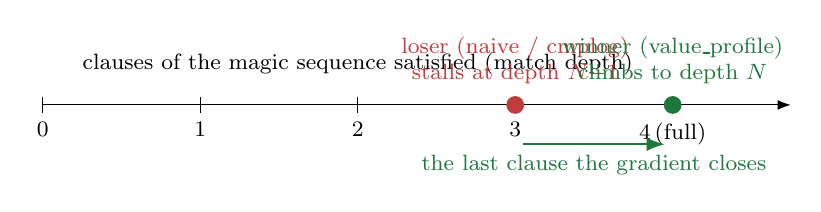
\begin{tikzpicture}[font=\footnotesize,>=Latex]
\draw[->] (0,0) -- (9.5,0);
\foreach \x/\l in {0/0, 2/1, 4/2, 6/3, 8/4\,(full)} \draw (\x,0.1)--(\x,-0.1) node[below]{\l};
\node[above] at (4,0.25) {clauses of the magic sequence satisfied (match depth)};
% loser stalls at N-1
\filldraw[losc] (6,0) circle (3pt) node[above=4pt,losc,align=center]{loser (naive / cmplog)\\stalls at depth $N{-}1$};
% winner reaches N
\filldraw[winc] (8,0) circle (3pt) node[above=4pt,winc,align=center]{winner (value\_profile)\\climbs to depth $N$};
\draw[->,winc,thick] (6.1,-0.5) -- (7.9,-0.5) node[midway,below]{the last clause the gradient closes};
\end{tikzpicture}\\[2pt]
{\footnotesize The conjunction climb: each \texttt{\&\&} clause is a step. The loser
gets within one byte (so it leaks coverage and dodges the $\ge 8/8$ filter), but
only value\_profile's per-clause gradient takes the final step.}
\end{center}

% =====================================================================
\section*{At a glance}
\begin{center}\small
\begin{tabular}{@{}p{3.8cm}clp{4.8cm}@{}}
\toprule
\textbf{Category} & \textbf{$n$} & \textbf{Tool / metric} & \textbf{One-line reason} \\
\midrule
operand byte-gradient climb & 33 & value\_distance\_reached (floating) / operand\_enrichment (fixed offset) & climb to the exact gate operand --- by distance, or by fixed-offset enrichment \\
assembly depth & 20 & depth\_reach (depth route) / struct\_size\_and\_token\_count (size route) & the gradient builds more structure --- drives the gate deeper per seed (depth), or admits a larger / token-denser corpus (size) \\
\midrule
\textbf{VP-pro total (auto-discovered)} & \textbf{53} & & \\
\midrule
incremental conjunction climb $\dagger$ & 7$^{*}$ & detect\_conjunction\_gate $+$ conjunction\_match\_depth & climb a multi-byte \texttt{\&\&} magic / BOM sequence clause-by-clause \\
\bottomrule
\end{tabular}
\end{center}

\noindent\footnotesize $\dagger$ \emph{Recovered} category (\S3): a false negative
of the auto-pipeline --- the strict $\ge 8/8$ admission filters out every
short-circuit-\texttt{\&\&} conjunction gate (the clause coverage leak depresses
\texttt{loser\_blocked}), so it never reached the classifier.
$^{*}$ 2 keyword conjunctions reclaimed from category~1 (\texttt{"ID"},
\texttt{"ANY"}) $+$ 5 BOM gates retrieved from libxml2 \texttt{xmlDetectCharEncoding}
by relaxed admission ($\ge 8$ / $\ge 4$) and confirmed by the match-depth arbiter;
the 5 are \emph{not} part of the 53 auto-discovered total, and a cross-target
census is pending.

\medskip\noindent\footnotesize Counts and example metrics regenerated from
\texttt{bench/dataset.jsonl} (cats 1--2) and the conjunction tools (cat~3);
verify rules are the deterministic arbiter rules (no LLM in the decision).
lcms/libxml2 gates are verified against local source dumps; harfbuzz/sqlite3
gates are from their analysis cards (their corpora live on the other server). The
common thread across all categories is the \emph{partial-match gradient}:
value\_profile turns a wrong/right cliff into a slope, which it then climbs ---
to the exact operand (1, by sliding-window distance for a floating operand or by
fixed-offset enrichment), by building more structure (2, driving the gate deeper
per seed or admitting a larger / token-denser corpus), or up a multi-byte
conjunction one clause at a time (3, the recovered category).
\end{document}
